\chapter{Greedy algorithms}

\index{ahne algoritmi@ahne algoritmi}

\key{Ahne algoritmi}
muodostaa tehtävän ratkaisun
tekemällä joka askeleella
sillä hetkellä parhaalta näyttävän valinnan.
Ahne algoritmi ei koskaan 
peruuta tekemiään valintoja vaan
muodostaa ratkaisun suoraan valmiiksi.
Tämän ansiosta ahneet algoritmit ovat
yleensä hyvin tehokkaita.

Vaikeutena ahneissa algoritmeissa on
keksiä toimiva ahne strategia,
joka tuottaa aina optimaalisen ratkaisun tehtävään.
Ahneen algoritmin tulee olla sellainen,
että kulloinkin parhaalta näyttävät valinnat
tuottavat myös parhaan kokonaisuuden.
Tämän perusteleminen on usein hankalaa.

\section{Kolikkotehtävä}

Aloitamme ahneisiin algoritmeihin tutustumisen
tehtävästä, jossa muodostettavana on
rahamäärä $x$ kolikoista.
Kolikoiden arvot ovat $\{c_1,c_2,\ldots,c_k\}$,
ja jokaista kolikkoa on saatavilla rajattomasti.
Tehtävänä on selvittää, mikä on pienin määrä
kolikoita, joilla rahamäärän voi muodostaa.

Esimerkiksi jos muodostettava
rahamäärä on 520
ja kolikot ovat eurokolikot eli sentteinä
\[\{1,2,5,10,20,50,100,200\},\]
niin kolikoita tarvitaan vähintään 4.
Tämä on mahdollista valitsemalla kolikot
$200+200+100+20$, joiden summa on 520.

\subsubsection{Ahne algoritmi}

Luonteva ahne algoritmi tehtävään
on poistaa rahamäärästä aina mahdollisimman
suuri kolikko, kunnes rahamäärä on 0.
Tämä algoritmi toimii esimerkissä,
koska rahamäärästä 520 
poistetaan ensin kahdesti 200, sitten 100
ja lopuksi 20.
Mutta toimiiko ahne algoritmi aina oikein?

Osoittautuu, että eurokolikoiden tapauksessa
ahne algoritmi \emph{toimii} aina oikein,
eli se tuottaa aina ratkaisun,
jossa on pienin määrä kolikoita.
Algoritmin toimivuuden voi perustella
seuraavasti:

Kutakin kolikkoa 1, 5, 10, 50 ja 100
on optimiratkaisussa enintään yksi.
Tämä johtuu siitä, että jos
ratkaisussa olisi kaksi tällaista kolikkoa,
saman ratkaisun voisi muodostaa
käyttäen vähemmän kolikoita.
Esimerkiksi jos ratkaisussa on
kolikot $5+5$, ne voi korvata kolikolla 10.

Vastaavasti kumpaakin kolikkoa 2 ja 20
on optimiratkaisussa enintään kaksi,
koska kolikot $2+2+2$ voi korvata kolikoilla $5+1$
ja kolikot $20+20+20$ voi korvata kolikoilla $50+10$.
Lisäksi ratkaisussa ei voi olla yhdistelmiä
$2+2+1$ ja $20+20+10$,
koska ne voi korvata kolikoilla 5 ja 50.

Näiden havaintojen perusteella
jokaiselle kolikolle $x$ pätee,
että $x$:ää pienemmistä kolikoista
ei ole mahdollista saada aikaan summaa
$x$ tai suurempaa summaa optimaalisesti.
Esimerkiksi jos $x=100$, pienemmistä kolikoista
saa korkeintaan summan $50+20+20+5+2+2=99$.
Niinpä ahne algoritmi,
joka valitsee aina suurimman kolikon,
tuottaa optimiratkaisun.

Kuten tästä esimerkistä huomaa,
ahneen algoritmin toimivuuden perusteleminen
voi olla työlästä,
vaikka kyseessä olisi yksinkertainen algoritmi.

\subsubsection{Yleinen tapaus}

Yleisessä tapauksessa kolikot voivat olla mitä tahansa.
Tällöin suurimman kolikon valitseva ahne algoritmi
\emph{ei} välttämättä tuota optimiratkaisua.

Jos ahne algoritmi ei toimi, tämän voi osoittaa
näyttämällä vastaesimerkin, jossa algoritmi
antaa väärän vastauksen.
Tässä tehtävässä vastaesimerkki on helppoa keksiä:
jos kolikot ovat $\{1,3,4\}$ ja muodostettava
rahamäärä on 6, ahne algoritmi tuottaa ratkaisun
$4+1+1$, kun taas optimiratkaisu on $3+3$.

Yleisessä tapauksessa kolikkotehtävän ratkaisuun
ei tunneta ahnetta algoritmia,
mutta palaamme tehtävään seuraavassa luvussa.
Tehtävään on nimittäin olemassa dynaamista
ohjelmointia käyttävä algoritmi,
joka tuottaa optimiratkaisun
millä tahansa kolikoilla ja rahamäärällä.

\section{Aikataulutus}

Monet aikataulutukseen liittyvät ongelmat
ratkeavat ahneesti.
Klassinen ongelma on seuraava:
Annettuna on $n$ tapahtumaa,
jotka alkavat ja päättyvät tiettyinä hetkinä.
Tehtäväsi on suunnitella aikataulu,
jota seuraamalla pystyt osallistumaan
mahdollisimman moneen tapahtumaan.
Et voi osallistua tapahtumaan vain osittain.
Esimerkiksi tilanteessa
\begin{center}
\begin{tabular}{lll}
tapahtuma & alkuaika & loppuaika \\
\hline
$A$ & 1 & 3 \\
$B$ & 2 & 5 \\
$C$ & 3 & 9 \\
$D$ & 6 & 8 \\
\end{tabular}
\end{center}
on mahdollista osallistua korkeintaan
kahteen tapahtumaan.
Yksi mahdollisuus on osallistua tapahtumiin
$B$ ja $D$ seuraavasti:
\begin{center}
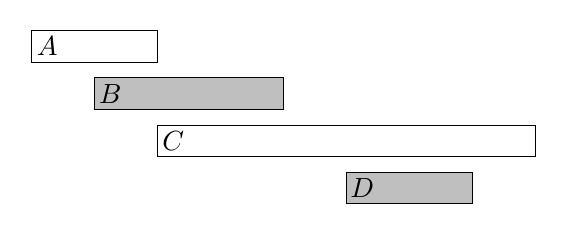
\begin{tikzpicture}[scale=.4]
  \begin{scope}
    \draw (2, 0) rectangle (6, -1);
    \draw[fill=lightgray] (4, -1.5) rectangle (10, -2.5);
    \draw (6, -3) rectangle (18, -4);
    \draw[fill=lightgray] (12, -4.5) rectangle (16, -5.5);
    \node at (2.5,-0.5) {$A$};
    \node at (4.5,-2) {$B$};
    \node at (6.5,-3.5) {$C$};
    \node at (12.5,-5) {$D$};
  \end{scope}
\end{tikzpicture}
\end{center}

Tehtävän ratkaisuun on mahdollista 
keksiä useita ahneita algoritmeja,
mutta mikä niistä toimii kaikissa tapauksissa?

\subsubsection*{Algoritmi 1}

Ensimmäinen idea on valita ratkaisuun
mahdollisimman \emph{lyhyitä} tapahtumia.
Esimerkin tapauksessa tällainen
algoritmi valitsee seuraavat tapahtumat:
\begin{center}
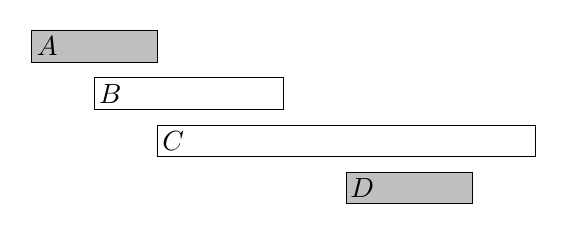
\begin{tikzpicture}[scale=.4]
  \begin{scope}
    \draw[fill=lightgray] (2, 0) rectangle (6, -1);
    \draw (4, -1.5) rectangle (10, -2.5);
    \draw (6, -3) rectangle (18, -4);
    \draw[fill=lightgray] (12, -4.5) rectangle (16, -5.5);
    \node at (2.5,-0.5) {$A$};
    \node at (4.5,-2) {$B$};
    \node at (6.5,-3.5) {$C$};
    \node at (12.5,-5) {$D$};
  \end{scope}
\end{tikzpicture}
\end{center}

Lyhimpien tapahtumien valinta ei ole kuitenkaan
aina toimiva strategia,
vaan algoritmi epäonnistuu esimerkiksi seuraavassa tilanteessa:
\begin{center}
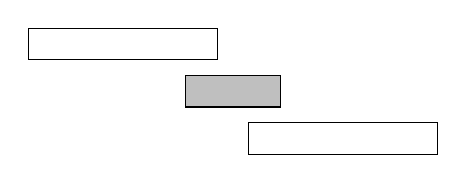
\begin{tikzpicture}[scale=.4]
  \begin{scope}
    \draw (1, 0) rectangle (7, -1);
    \draw[fill=lightgray] (6, -1.5) rectangle (9, -2.5);
    \draw (8, -3) rectangle (14, -4);
  \end{scope}
\end{tikzpicture}
\end{center}
Kun lyhyt tapahtuma valitaan mukaan,
on mahdollista osallistua vain yhteen tapahtumaan.
Kuitenkin valitsemalla pitkät tapahtumat
olisi mahdollista osallistua kahteen tapahtumaan.

\subsubsection*{Algoritmi 2}

Toinen idea on valita aina seuraavaksi tapahtuma,
joka \emph{alkaa} mahdollisimman aikaisin.
Tämä algoritmi valitsee esimerkissä seuraavat tapahtumat:
\begin{center}
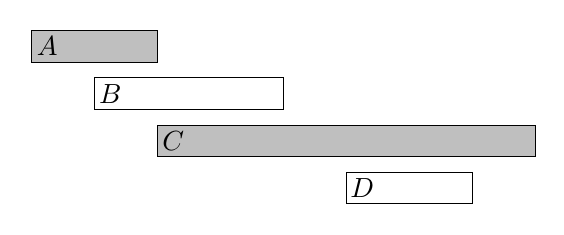
\begin{tikzpicture}[scale=.4]
  \begin{scope}
    \draw[fill=lightgray] (2, 0) rectangle (6, -1);
    \draw (4, -1.5) rectangle (10, -2.5);
    \draw[fill=lightgray] (6, -3) rectangle (18, -4);
    \draw (12, -4.5) rectangle (16, -5.5);
    \node at (2.5,-0.5) {$A$};
    \node at (4.5,-2) {$B$};
    \node at (6.5,-3.5) {$C$};
    \node at (12.5,-5) {$D$};
  \end{scope}
\end{tikzpicture}
\end{center}

Tämäkään algoritmi ei kuitenkaan toimi aina.
Esimerkiksi seuraavassa tilanteessa
algoritmi valitsee vain yhden tapahtuman:
\begin{center}
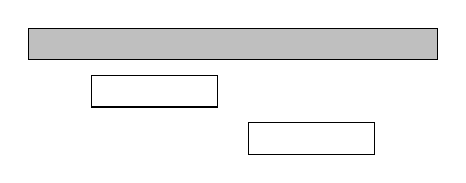
\begin{tikzpicture}[scale=.4]
  \begin{scope}
    \draw[fill=lightgray] (1, 0) rectangle (14, -1);
    \draw (3, -1.5) rectangle (7, -2.5);
    \draw (8, -3) rectangle (12, -4);
  \end{scope}
\end{tikzpicture}
\end{center}
Kun ensimmäisenä alkava tapahtuma
valitaan mukaan, mitään muuta tapahtumaa
ei ole mahdollista valita.
Kuitenkin olisi mahdollista osallistua
kahteen tapahtumaan valitsemalla
kaksi myöhempää tapahtumaa.

\subsubsection*{Algoritmi 3}

Kolmas idea on valita aina seuraavaksi tapahtuma,
joka \emph{päättyy} mahdollisimman aikaisin.
Tämä algoritmi valitsee esimerkissä seuraavat tapahtumat:
\begin{center}
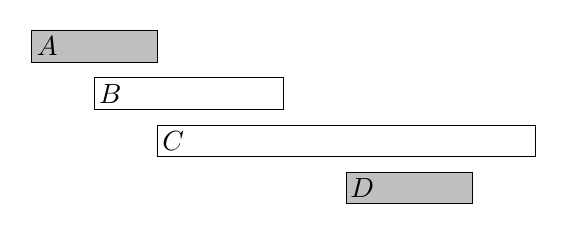
\begin{tikzpicture}[scale=.4]
  \begin{scope}
    \draw[fill=lightgray] (2, 0) rectangle (6, -1);
    \draw (4, -1.5) rectangle (10, -2.5);
    \draw (6, -3) rectangle (18, -4);
    \draw[fill=lightgray] (12, -4.5) rectangle (16, -5.5);
    \node at (2.5,-0.5) {$A$};
    \node at (4.5,-2) {$B$};
    \node at (6.5,-3.5) {$C$};
    \node at (12.5,-5) {$D$};
  \end{scope}
\end{tikzpicture}
\end{center}

Osoittautuu, että tämä ahne algoritmi
tuottaa \textit{aina} optimiratkaisun.
Algoritmi toimii, koska on aina kokonaisuuden
kannalta optimaalista valita
ensimmäiseksi tapahtumaksi
mahdollisimman aikaisin päättyvä tapahtuma.
Tämän jälkeen on taas optimaalista
valita seuraava aikatauluun sopiva
mahdollisimman aikaisin
päättyvä tapahtua, jne.

Yksi tapa perustella valintaa on miettiä,
mitä tapahtuu, jos ensimmäiseksi tapahtumaksi
valitaan jokin muu kuin mahdollisimman
aikaisin päättyvä tapahtuma.
Tällainen valinta ei ole koskaan parempi,
koska myöhemmin päättyvän tapahtuman
jälkeen on joko yhtä paljon tai vähemmän
mahdollisuuksia valita seuraavia tapahtumia
kuin aiemmin päättyvän tapahtuman jälkeen.

\section{Tehtävät ja deadlinet}

Annettuna on $n$ tehtävää,
joista jokaisella on kesto ja deadline.
Tehtäväsi on valita järjestys,
jossa suoritat tehtävät.
Saat kustakin tehtävästä $d-x$ pistettä,
missä $d$ on tehtävän deadline ja $x$
on tehtävän valmistumishetki.
Mikä on suurin mahdollinen
yhteispistemäärä, jonka voit saada tehtävistä?

Esimerkiksi jos tehtävät ovat
\begin{center}
\begin{tabular}{lll}
tehtävä & kesto & deadline \\
\hline
$A$ & 4 & 2 \\
$B$ & 3 & 5 \\
$C$ & 2 & 7 \\
$D$ & 4 & 5 \\
\end{tabular}
\end{center}
niin optimaalinen ratkaisu on suorittaa
tehtävät seuraavasti:
\begin{center}
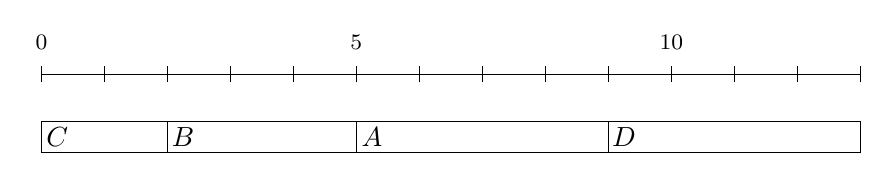
\begin{tikzpicture}[scale=.4]
  \begin{scope}
    \draw (0, 0) rectangle (4, -1);
    \draw (4, 0) rectangle (10, -1);
    \draw (10, 0) rectangle (18, -1);
    \draw (18, 0) rectangle (26, -1);
    \node at (0.5,-0.5) {$C$};
    \node at (4.5,-0.5) {$B$};
    \node at (10.5,-0.5) {$A$};
    \node at (18.5,-0.5) {$D$};

    \draw (0,1.5) -- (26,1.5);
    \foreach \i in {0,2,...,26}
    {
        \draw (\i,1.25) -- (\i,1.75);
    }
    \footnotesize
    \node at (0,2.5) {0};
    \node at (10,2.5) {5};
    \node at (20,2.5) {10};

  \end{scope}
\end{tikzpicture}
\end{center}
Tässä ratkaisussa $C$ tuottaa 5 pistettä,
$B$ tuottaa 0 pistettä, $A$ tuottaa $-7$ pistettä
ja $D$ tuottaa $-8$ pistettä,
joten yhteispistemäärä on $-10$.

Yllättävää kyllä, tehtävän optimaalinen ratkaisu
ei riipu lainkaan deadlineista,
vaan toimiva ahne strategia on
yksinkertaisesti
suorittaa tehtävät \emph{järjestyksessä keston mukaan}
lyhimmästä pisimpään.
Syynä tähän on, että jos missä tahansa vaiheessa
suoritetaan peräkkäin kaksi tehtävää,
joista ensimmäinen kestää toista kauemmin,
tehtävien järjestyksen vaihtaminen parantaa ratkaisua.
Esimerkiksi jos peräkkäin ovat tehtävät
\begin{center}
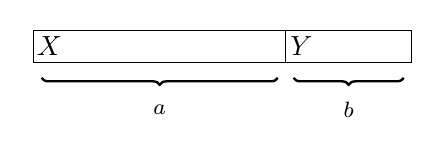
\begin{tikzpicture}[scale=.4]
  \begin{scope}
    \draw (0, 0) rectangle (8, -1);
    \draw (8, 0) rectangle (12, -1);
    \node at (0.5,-0.5) {$X$};
    \node at (8.5,-0.5) {$Y$};

\draw [decoration={brace}, decorate, line width=0.3mm] (7.75,-1.5) -- (0.25,-1.5);
\draw [decoration={brace}, decorate, line width=0.3mm] (11.75,-1.5) -- (8.25,-1.5);

\footnotesize
\node at (4,-2.5) {$a$};
\node at (10,-2.5) {$b$};

  \end{scope}
\end{tikzpicture}
\end{center}
ja $a>b$, niin järjestyksen muuttaminen muotoon
\begin{center}
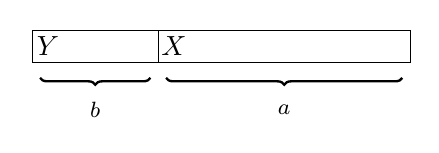
\begin{tikzpicture}[scale=.4]
  \begin{scope}
    \draw (0, 0) rectangle (4, -1);
    \draw (4, 0) rectangle (12, -1);
    \node at (0.5,-0.5) {$Y$};
    \node at (4.5,-0.5) {$X$};

\draw [decoration={brace}, decorate, line width=0.3mm] (3.75,-1.5) -- (0.25,-1.5);
\draw [decoration={brace}, decorate, line width=0.3mm] (11.75,-1.5) -- (4.25,-1.5);

\footnotesize
\node at (2,-2.5) {$b$};
\node at (8,-2.5) {$a$};

  \end{scope}
\end{tikzpicture}
\end{center}
antaa $X$:lle $b$ pistettä vähemmän ja $Y$:lle $a$ pistettä enemmän,
joten kokonaismuutos pistemäärään on $a-b > 0$.
Optimiratkaisussa
kaikille peräkkäin suoritettaville tehtäville
tulee päteä, että lyhyempi tulee ennen pidempää,
mistä seuraa, että tehtävät tulee suorittaa
järjestyksessä keston mukaan.

\section{Keskiluvut}

Tarkastelemme seuraavaksi ongelmaa, jossa
annettuna on $n$ lukua $a_1,a_2,\ldots,a_n$
ja tehtävänä on etsiä luku $x$ niin, että summa
\[|a_1-x|^c+|a_2-x|^c+\cdots+|a_n-x|^c\]
on mahdollisimman pieni.
Keskitymme tapauksiin, joissa $c=1$ tai $c=2$.

\subsubsection{Tapaus $c=1$}

Tässä tapauksessa minimoitavana on summa
\[|a_1-x|+|a_2-x|+\cdots+|a_n-x|.\]
Esimerkiksi jos luvut ovat $[1,2,9,2,6]$,
niin paras ratkaisu on valita $x=2$,
jolloin summaksi tulee
\[
|1-2|+|2-2|+|9-2|+|2-2|+|6-2|=12.
\]
Yleisessä tapauksessa paras valinta $x$:n arvoksi
on lukujen \textit{mediaani}
eli keskimmäinen luku järjestyksessä.
Esimerkiksi luvut $[1,2,9,2,6]$
ovat järjestyksessä $[1,2,2,6,9]$,
joten mediaani on 2.

Mediaanin valinta on paras ratkaisu,
koska jos $x$ on mediaania pienempi,
$x$:n suurentaminen pienentää summaa,
ja vastaavasti jos $x$ on mediaania suurempi,
$x$:n pienentäminen pienentää summaa.
Niinpä $x$ kannattaa siirtää mahdollisimman
lähelle mediaania eli optimiratkaisu on
valita $x$ mediaaniksi.
Jos $n$ on parillinen ja mediaaneja on kaksi,
kumpikin mediaani sekä kaikki niiden välillä
olevat luvut tuottavat optimaalisen ratkaisun.

\subsubsection{Tapaus $c=2$}

Tässä tapauksessa minimoitavana on summa
\[(a_1-x)^2+(a_2-x)^2+\cdots+(a_n-x)^2.\]
Esimerkiksi jos luvut ovat $[1,2,9,2,6]$,
niin paras ratkaisu on $x=4$,
jolloin summaksi tulee
\[
(1-4)^2+(2-4)^2+(9-4)^2+(2-4)^2+(6-4)^2=46.
\]
Yleisessä tapauksessa paras valinta $x$:n arvoksi on lukujen
\textit{keskiarvo}.
Esimerkissä lukujen keskiarvo on $(1+2+9+2+6)/5=4$.
Tämän tuloksen voi johtaa järjestämällä summan
uudestaan muotoon
\[
nx^2 - 2x(a_1+a_2+\cdots+a_n) + (a_1^2+a_2^2+\cdots+a_n^2).
\]
Viimeinen osa ei riipu $x$:stä, joten sen voi jättää huomiotta.
Jäljelle jäävistä osista muodostuu funktio
$nx^2-2xs$, kun $s=a_1+a_2+\cdots+a_n$.
Tämä on ylöspäin aukeava paraabeli,
jonka nollakohdat ovat $x=0$ ja $x=2s/n$
ja pienin arvo on näiden keskikohta
$x=s/n$ eli taulukon lukujen keskiarvo.

\section{Tiedonpakkaus}

\index{tiedonpakkaus}
\index{binxxrikoodi@binäärikoodi}
\index{koodisana@koodisana}

Annettuna on merkkijono ja tehtävänä on
\emph{pakata} se niin,
että tilaa kuluu vähemmän.
Käytämme tähän \key{binäärikoodia},
joka määrittää kullekin merkille
biteistä muodostuvan \key{koodisanan}.
Tällöin merkkijonon voi pakata
korvaamalla jokaisen merkin vastaavalla koodisanalla.
Esimerkiksi seuraava binäärikoodi määrittää
koodisanat merkeille \texttt{A}–\texttt{D}:
\begin{center}
\begin{tabular}{rr}
merkki & koodisana \\
\hline
\texttt{A} & 00 \\
\texttt{B} & 01 \\
\texttt{C} & 10 \\
\texttt{D} & 11 \\
\end{tabular}
\end{center}
Tämä koodi on \key{vakiopituinen}
eli jokainen koodisana on yhtä pitkä.
Esimerkiksi merkkijono
\texttt{AABACDACA} on pakattuna
\[000001001011001000,\]
eli se vie tilaa 18 bittiä.
Pakkausta on kuitenkin mahdollista parantaa
ottamalla käyttöön \key{muuttuvan pituinen} koodi,
jossa koodisanojen pituus voi vaihdella.
Tällöin voimme antaa usein esiintyville merkeille
lyhyen koodisanan ja harvoin esiintyville
merkeille pitkän koodisanan.
Osoittautuu, että yllä olevalle merkkijonolle
\key{optimaalinen} koodi on seuraava:
\begin{center}
\begin{tabular}{rr}
merkki & koodisana \\
\hline
\texttt{A} & 0 \\
\texttt{B} & 110 \\
\texttt{C} & 10 \\
\texttt{D} & 111 \\
\end{tabular}
\end{center}
Optimaalinen koodi tuottaa
mahdollisimman lyhyen pakatun merkkijonon.
Tässä tapauksessa optimaalinen koodi
pakkaa merkkijonon muotoon
\[001100101110100,\]
ja tilaa kuluu vain 15 bittiä.
Paremman koodin ansiosta onnistuimme siis säästämään
3 bittiä tilaa pakkauksessa.

Huomaa, että koodin tulee olla aina sellainen,
että mikään koodisana ei ole toisen koodisanan
alkuosa.
Esimerkiksi ei ole sallittua, että koodissa
olisi molemmat koodisanat 10 ja 1011.
Tämä rajoitus johtuu siitä,
että haluamme myös pystyä palauttamaan
alkuperäisen merkkijonon pakkauksen jälkeen.
Jos koodisana voisi olla toisen alkuosa,
tämä ei välttämättä olisi mahdollista.
Esimerkiksi seuraava koodi
\emph{ei} ole kelvollinen:
\begin{center}
\begin{tabular}{rr}
merkki & koodisana \\
\hline
\texttt{A} & 10 \\
\texttt{B} & 11 \\
\texttt{C} & 1011 \\
\texttt{D} & 111 \\
\end{tabular}
\end{center}
Tätä koodia käyttäen ei olisi mahdollista tietää,
tarkoittaako pakattu merkkijono 1011
merkkijonoa \texttt{AB} vai merkkijonoa \texttt{C}.

\index{Huffmanin koodaus}

\subsubsection{Huffmanin koodaus}

\key{Huffmanin koodaus} on ahne algoritmi,
joka muodostaa optimaalisen koodin
merkkijonon pakkaamista varten.
Se muodostaa merkkien esiintymiskertojen
perustella binääripuun, josta voi lukea
kunkin merkin koodisanan
liikkumalla huipulta merkkiä vastaavaan solmuun.
Liikkuminen vasemmalle vastaa
bittiä 0 ja liikkuminen oikealle
vastaa bittiä 1.

Aluksi jokaista merkkijonon merkkiä vastaa solmu,
jonka painona on merkin esiintymiskertojen määrä merkkijonossa.
Sitten joka vaiheessa puusta valitaan
kaksi painoltaan pienintä solmua
ja ne yhdistetään luomalla niiden
yläpuolelle uusi solmu,
jonka paino on solmujen yhteispaino.
Näin jatketaan, kunnes kaikki solmut
on yhdistetty ja koodi on valmis.

Tarkastellaan nyt, miten Huffmanin koodaus
muodostaa optimaalisen koodin merkkijonolle
\texttt{AABACDACA}.
Alkutilanteessa on neljä solmua,
jotka vastaavat merkkijonossa olevia merkkejä:

\begin{center}
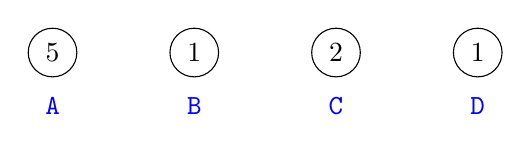
\begin{tikzpicture}[scale=0.9]
\node[draw, circle] (1) at (0,0) {$5$};
\node[draw, circle] (2) at (2,0) {$1$};
\node[draw, circle] (3) at (4,0) {$2$};
\node[draw, circle] (4) at (6,0) {$1$};

\node[color=blue] at (0,-0.75) {\texttt{A}};
\node[color=blue] at (2,-0.75) {\texttt{B}};
\node[color=blue] at (4,-0.75) {\texttt{C}};
\node[color=blue] at (6,-0.75) {\texttt{D}};

%\path[draw,thick,-] (4) -- (5);
\end{tikzpicture}
\end{center}
Merkkiä \texttt{A} vastaavan solmun paino on
5, koska merkki \texttt{A} esiintyy 5 kertaa merkkijonossa.
Muiden solmujen painot on laskettu vastaavalla tavalla.

Ensimmäinen askel on yhdistää merkkejä \texttt{B} ja \texttt{D}
vastaavat solmut, joiden kummankin paino on 1.
Tuloksena on:
\begin{center}
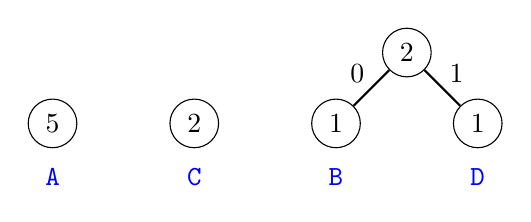
\begin{tikzpicture}[scale=0.9]
\node[draw, circle] (1) at (0,0) {$5$};
\node[draw, circle] (3) at (2,0) {$2$};
\node[draw, circle] (2) at (4,0) {$1$};
\node[draw, circle] (4) at (6,0) {$1$};
\node[draw, circle] (5) at (5,1) {$2$};

\node[color=blue] at (0,-0.75) {\texttt{A}};
\node[color=blue] at (2,-0.75) {\texttt{C}};
\node[color=blue] at (4,-0.75) {\texttt{B}};
\node[color=blue] at (6,-0.75) {\texttt{D}};

\node at (4.3,0.7) {0};
\node at (5.7,0.7) {1};

\path[draw,thick,-] (2) -- (5);
\path[draw,thick,-] (4) -- (5);
\end{tikzpicture}
\end{center}
Tämän jälkeen yhdistetään solmut, joiden paino on 2:
\begin{center}
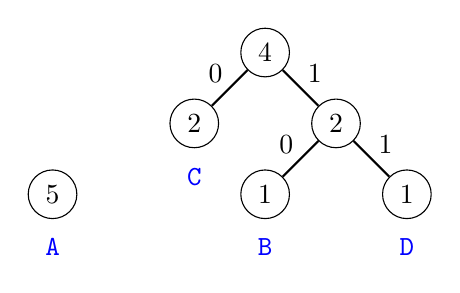
\begin{tikzpicture}[scale=0.9]
\node[draw, circle] (1) at (1,0) {$5$};
\node[draw, circle] (3) at (3,1) {$2$};
\node[draw, circle] (2) at (4,0) {$1$};
\node[draw, circle] (4) at (6,0) {$1$};
\node[draw, circle] (5) at (5,1) {$2$};
\node[draw, circle] (6) at (4,2) {$4$};

\node[color=blue] at (1,-0.75) {\texttt{A}};
\node[color=blue] at (3,1-0.75) {\texttt{C}};
\node[color=blue] at (4,-0.75) {\texttt{B}};
\node[color=blue] at (6,-0.75) {\texttt{D}};

\node at (4.3,0.7) {0};
\node at (5.7,0.7) {1};
\node at (3.3,1.7) {0};
\node at (4.7,1.7) {1};

\path[draw,thick,-] (2) -- (5);
\path[draw,thick,-] (4) -- (5);
\path[draw,thick,-] (3) -- (6);
\path[draw,thick,-] (5) -- (6);
\end{tikzpicture}
\end{center}
Lopuksi yhdistetään kaksi viimeistä solmua:
\begin{center}
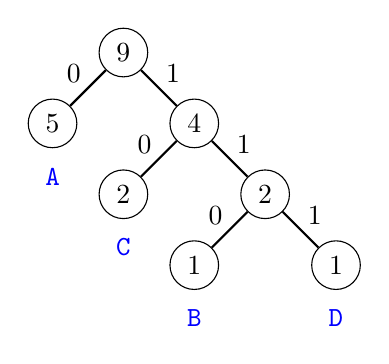
\begin{tikzpicture}[scale=0.9]
\node[draw, circle] (1) at (2,2) {$5$};
\node[draw, circle] (3) at (3,1) {$2$};
\node[draw, circle] (2) at (4,0) {$1$};
\node[draw, circle] (4) at (6,0) {$1$};
\node[draw, circle] (5) at (5,1) {$2$};
\node[draw, circle] (6) at (4,2) {$4$};
\node[draw, circle] (7) at (3,3) {$9$};

\node[color=blue] at (2,2-0.75) {\texttt{A}};
\node[color=blue] at (3,1-0.75) {\texttt{C}};
\node[color=blue] at (4,-0.75) {\texttt{B}};
\node[color=blue] at (6,-0.75) {\texttt{D}};

\node at (4.3,0.7) {0};
\node at (5.7,0.7) {1};
\node at (3.3,1.7) {0};
\node at (4.7,1.7) {1};
\node at (2.3,2.7) {0};
\node at (3.7,2.7) {1};

\path[draw,thick,-] (2) -- (5);
\path[draw,thick,-] (4) -- (5);
\path[draw,thick,-] (3) -- (6);
\path[draw,thick,-] (5) -- (6);
\path[draw,thick,-] (1) -- (7);
\path[draw,thick,-] (6) -- (7);
\end{tikzpicture}
\end{center}

Nyt kaikki solmut ovat puussa, joten koodi on valmis.
Puusta voidaan lukea seuraavat koodisanat:
\begin{center}
\begin{tabular}{rr}
merkki & koodisana \\
\hline
\texttt{A} & 0 \\
\texttt{B} & 110 \\
\texttt{C} & 10 \\
\texttt{D} & 111 \\
\end{tabular}
\end{center}

% \subsubsection{Miksi algoritmi toimii?}
% 
% Huffmanin koodaus on ahne algoritmi, koska se
% yhdistää aina kaksi solmua, joiden painot ovat
% pienimmät.
% Miksi on varmaa, että tämä menetelmä tuottaa
% aina optimaalisen koodin?
% 
% Merkitään $c(x)$ merkin $x$ esiintymiskertojen
% määrää merkkijonossa sekä $s(x)$
% merkkiä $x$ vastaavan koodisanan pituutta.
% Näitä merkintöjä käyttäen merkkijonon
% bittiesityksen pituus on
% \[\sum_x c(x) \cdot s(x),\]
% missä summa käy läpi kaikki merkkijonon merkit.
% Esimerkiksi äskeisessä esimerkissä
% bittiesityksen pituus on
% \[5 \cdot 1 + 1 \cdot 3 + 2 \cdot 2 + 1 \cdot 3 = 15.\]
% Hyödyllinen havainto on, että $s(x)$ on yhtä suuri kuin
% merkkiä $x$ vastaavan solmun \emph{syvyys} puussa
% eli matka puun huipulta solmuun.
% 
% Perustellaan ensin, miksi optimaalista koodia vastaa
% aina binääripuu, jossa jokaisesta solmusta lähtee
% alaspäin joko kaksi haaraa tai ei yhtään haaraa.
% Tehdään vastaoletus, että jostain solmusta lähtisi
% alaspäin vain yksi haara.
% Esimerkiksi seuraavassa puussa tällainen tilanne on solmussa $a$:
% \begin{center}
% \begin{tikzpicture}[scale=0.9]
% \node[draw, circle, minimum size=20pt] (3) at (3,1) {\phantom{$a$}};
% \node[draw, circle, minimum size=20pt] (2) at (4,0) {$b$};
% \node[draw, circle, minimum size=20pt] (5) at (5,1) {$a$};
% \node[draw, circle, minimum size=20pt] (6) at (4,2) {\phantom{$a$}};
% 
% \path[draw,thick,-] (2) -- (5);
% \path[draw,thick,-] (3) -- (6);
% \path[draw,thick,-] (5) -- (6);
% \end{tikzpicture}
% \end{center}
% Tällainen solmu $a$ on kuitenkin aina turha, koska se
% tuo vain yhden bitin lisää polkuihin, jotka kulkevat
% solmun kautta, eikä sen avulla voi erottaa kahta
% koodisanaa toisistaan. Niinpä kyseisen solmun voi poistaa
% puusta, minkä seurauksena syntyy parempi koodi,
% eli optimaalista koodia vastaavassa puussa ei voi olla
% solmua, josta lähtee vain yksi haara.
% 
% Perustellaan sitten, miksi on joka vaiheessa optimaalista
% yhdistää kaksi solmua, joiden painot ovat pienimmät.
% Tehdään vastaoletus, että solmun $a$ paino on pienin,
% mutta sitä ei saisi yhdistää aluksi toiseen solmuun,
% vaan sen sijasta tulisi yhdistää solmu $b$
% ja jokin toinen solmu:
% \begin{center}
% \begin{tikzpicture}[scale=0.9]
% \node[draw, circle, minimum size=20pt] (1) at (0,0) {\phantom{$a$}};
% \node[draw, circle, minimum size=20pt] (2) at (-2,-1) {\phantom{$a$}};
% \node[draw, circle, minimum size=20pt] (3) at (2,-1) {$a$};
% \node[draw, circle, minimum size=20pt] (4) at (-3,-2) {\phantom{$a$}};
% \node[draw, circle, minimum size=20pt] (5) at (-1,-2) {\phantom{$a$}};
% \node[draw, circle, minimum size=20pt] (8) at (-2,-3) {$b$};
% \node[draw, circle, minimum size=20pt] (9) at (0,-3) {\phantom{$a$}};
% 
% \path[draw,thick,-] (1) -- (2);
% \path[draw,thick,-] (1) -- (3);
% \path[draw,thick,-] (2) -- (4);
% \path[draw,thick,-] (2) -- (5);
% \path[draw,thick,-] (5) -- (8);
% \path[draw,thick,-] (5) -- (9);
% \end{tikzpicture}
% \end{center}
% Solmuille $a$ ja $b$ pätee
% $c(a) \le c(b)$ ja $s(a) \le s(b)$.
% Solmut aiheuttavat bittiesityksen pituuteen lisäyksen
% \[c(a) \cdot s(a) + c(b) \cdot s(b).\]
% Tarkastellaan sitten toista tilannetta,
% joka on muuten samanlainen kuin ennen,
% mutta solmut $a$ ja $b$ on vaihdettu keskenään:
% \begin{center}
% \begin{tikzpicture}[scale=0.9]
% \node[draw, circle, minimum size=20pt] (1) at (0,0) {\phantom{$a$}};
% \node[draw, circle, minimum size=20pt] (2) at (-2,-1) {\phantom{$a$}};
% \node[draw, circle, minimum size=20pt] (3) at (2,-1) {$b$};
% \node[draw, circle, minimum size=20pt] (4) at (-3,-2) {\phantom{$a$}};
% \node[draw, circle, minimum size=20pt] (5) at (-1,-2) {\phantom{$a$}};
% \node[draw, circle, minimum size=20pt] (8) at (-2,-3) {$a$};
% \node[draw, circle, minimum size=20pt] (9) at (0,-3) {\phantom{$a$}};
% 
% \path[draw,thick,-] (1) -- (2);
% \path[draw,thick,-] (1) -- (3);
% \path[draw,thick,-] (2) -- (4);
% \path[draw,thick,-] (2) -- (5);
% \path[draw,thick,-] (5) -- (8);
% \path[draw,thick,-] (5) -- (9);
% \end{tikzpicture}
% \end{center}
% Osoittautuu, että tätä puuta vastaava koodi on
% \emph{yhtä hyvä tai parempi} kuin alkuperäinen koodi, joten vastaoletus
% on väärin ja Huffmanin koodaus
% toimiikin oikein, jos se yhdistää aluksi solmun $a$
% jonkin solmun kanssa.
% Tämän perustelee seuraava epäyhtälöketju:
% \[\begin{array}{rcl}
% c(b) & \ge & c(a) \\
% c(b)\cdot(s(b)-s(a)) & \ge & c(a)\cdot (s(b)-s(a)) \\
% c(b)\cdot s(b)-c(b)\cdot s(a) & \ge & c(a)\cdot s(b)-c(a)\cdot s(a) \\
% c(a)\cdot s(a)+c(b)\cdot s(b) & \ge & c(a)\cdot s(b)+c(b)\cdot s(a) \\
% \end{array}\]